\documentclass[12pt]{ltjsarticle}

% 基本パッケージ
\usepackage[utf8]{inputenc}
\usepackage{luatexja}
\usepackage{amsmath, amssymb}
\usepackage{graphicx}
\usepackage{geometry}

% 表のデザインを向上させるパッケージ
\usepackage{tikz}
\usetikzlibrary{arrows.meta, positioning}
\usepackage{booktabs}
\usepackage{tabularx}
\usepackage{longtable}
\usepackage{array}
\usepackage{makecell}

% セクションやタイトルのデザイン調整
\usepackage{titlesec}
\titleformat{\section}{\normalfont\Large\bfseries}{\thesection}{1em}{}
\titleformat{\subsection}{\normalfont\large\bfseries}{\thesubsection}{1em}{}
\titleformat{\subsubsection}{\normalfont\normalsize\bfseries}{\thesubsubsection}{1em}{}

\usepackage{enumitem}
\usepackage{fontspec}

\usepackage[
  colorlinks=true,
  linkcolor=blue,
  urlcolor=cyan,
  citecolor=green
]{hyperref}

\usepackage{listing}
\usepackage{xcolor}
\newcommand{\code}[1]{\colorbox{gray!20}{\texttt{#1}}}
\usepackage{float}
\geometry{top=2cm, bottom=2cm, left=2cm, right=2cm}
\usepackage{minted}

\usemintedstyle{vs}
\setminted{
    linenos,
    frame=single,
    framesep=2mm,
    baselinestretch=1.2,
    fontsize=\small,
    breaklines
}

% 数式
\usepackage{bm}

% 画像
\usepackage{float}

\begin{document}

\title{SportEase（スポーティーズ） admin操作説明書}
\author{行事委員会 佐藤佑作 s2301059}
\date{\today}
\maketitle
\tableofcontents

\newpage

% =====================================================================
\section{はじめに}
% =====================================================================

本書は、SportEase（スポーティーズ）の\textbf{admin権限を持つ運営スタッフ}向けの操作説明書である。
adminアカウントは大会当日の運営補助を主な役割とし、試合進行・結果入力・参加者管理など
競技運営に必要な操作を行うことができる。

\subsection*{権限の種類}
\begin{itemize}
  \item \textbf{root} ── 最上位権限。大会設定・システム管理・ユーザー管理など全機能にアクセス可能。
  \item \textbf{admin} ── 本書が対象とする権限。大会運営機能に加え、student向け機能にもアクセス可能。
  \item \textbf{student} ── マイページ・競技情報・トーナメント・通知などの参加者向け機能を利用できる基本権限。
\end{itemize}

基本権限である \code{root} / \code{admin} / \code{student} の付与・剥奪は
root専用の「権限管理」画面で行う。
一方、adminの「ロール管理」画面では審判ロールなどの任意ロールのみを扱う。

adminダッシュボードは \code{/dashboard/admin/} 以下の各ページから操作する。
admin権限を持たないアカウントでアクセスしようとした場合は、自動的に \code{/dashboard} へリダイレクトされる。

\subsection{admin作業時の基本方針}

adminは大会当日の進行に関わる操作を担当する。
試合ステータス、試合結果、出席者数、昼競技結果などは他画面に即時反映されるため、
入力前に対象大会・対象競技・対象クラスを必ず確認する。

\begin{center}
\begin{tabular}{p{4cm}p{9cm}}
\toprule
\textbf{確認項目} & \textbf{確認内容} \\
\midrule
対象大会 & 現在activeの大会が、当日運用している大会と一致しているか確認する。 \\
\midrule
担当範囲 & 自分が担当する競技・クラス・受付場所を事前に確認する。 \\
\midrule
入力根拠 & 試合結果や出席者数は、審判・担当者の確認後に入力する。 \\
\midrule
修正時の共有 & 一度登録した結果を修正する場合は、関係者に変更内容を共有する。 \\
\bottomrule
\end{tabular}
\end{center}

\subsection{大会当日の業務フロー}

大会当日のadmin業務は、以下の順序で進めることを推奨する。
各手順の詳細は対応するセクションを参照すること。
なお、MyIDバーコード読み取りによる参加本登録・ラウンドチェックインは、
必要に応じて実施する任意の操作である。

\begin{center}
\begin{tikzpicture}[
  node distance=1.3cm,
  main/.style={
    rectangle, draw, rounded corners=4pt,
    minimum width=9cm, minimum height=0.9cm,
    text centered, fill=blue!8, font=\bfseries
  },
  opt/.style={
    rectangle, draw, dashed, rounded corners=4pt,
    minimum width=4.5cm, minimum height=0.9cm,
    text centered, fill=gray!8, font=\bfseries
  },
  arr/.style={->, thick, >=Stealth},
  optarr/.style={->, dashed, >=Stealth}
]
\node[main] (s1) {① ログイン・ダッシュボード確認　→ 第\ref{sec:dashboard}章};
\node[main, below of=s1] (s2) {② ロール確認・事前準備　→ 第\ref{sec:role}章};
\node[main, below of=s2] (s3) {③ 出席者数の登録　→ 第\ref{sec:attendance}章};
\node[main, below of=s3] (s4) {④ 試合ステータス更新・結果入力　→ 第\ref{sec:match}章};
\node[main, below of=s4] (s5) {⑤ 昼競技結果入力　→ 第\ref{sec:noon}章};
\node[main, below of=s5] (s6) {⑥ MIC投票　→ 第\ref{sec:mic}章};

\node[opt, right=1.5cm of s3] (myid) {MyID読み取り（任意）→ 第\ref{sec:myid}章};

\draw[arr] (s1) -- (s2);
\draw[arr] (s2) -- (s3);
\draw[arr] (s3) -- (s4);
\draw[arr] (s4) -- (s5);
\draw[arr] (s5) -- (s6);
\draw[optarr] (s3.east) -- (myid.west);

\end{tikzpicture}
\end{center}

\subsection{初回ログイン}

\href{https://nitsche-gyouji.com}{https://nitsche-gyouji.com} をお好みのブラウザで開いてください。
すると、以下のような画面にアクセスできます。

\begin{figure}[H]
  \centering
  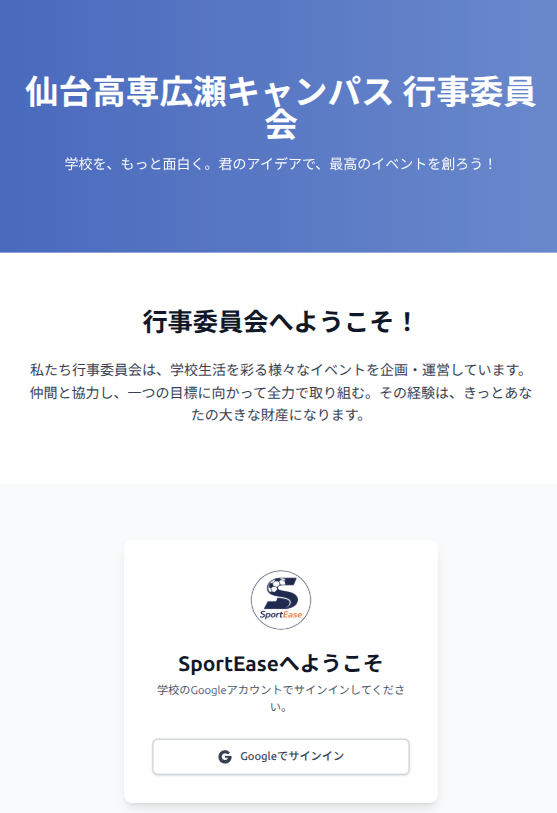
\includegraphics[width=0.8\textwidth]{./images/HP_first.png}
  \caption{アクセス結果}
\end{figure}

\texttt{Googleでサインイン}をクリックしてください。\\
\textcolor{red}{※学校のGoogle アカウントを必ず選択してください。学校のアカウント以外を選択してしまった場合は、ブラウザのキャッシュをクリアして再度アクセスしてください。}

サインインが成功すると、以下のように表示名とクラスを設定する画面に移ります。

\begin{figure}[H]
  \centering
  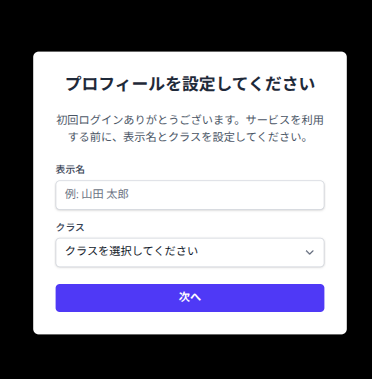
\includegraphics[width=0.8\textwidth]{./images/set-display-name.png}
  \caption{表示名とクラス設定画面}
\end{figure}

ここで、アプリ内での表示名とクラスを決定してください。
確認画面も表示されるので、クラスに関しては間違えないようにお願いします。

\newpage

% =====================================================================
\section{管理者ダッシュボード}\label{sec:dashboard}
% =====================================================================

\textbf{ページ}: \code{/dashboard/admin/manage-dashboard}

大会運営の状況をリアルタイムで把握するための統計ダッシュボードである。

\begin{figure}[H]
  \centering
  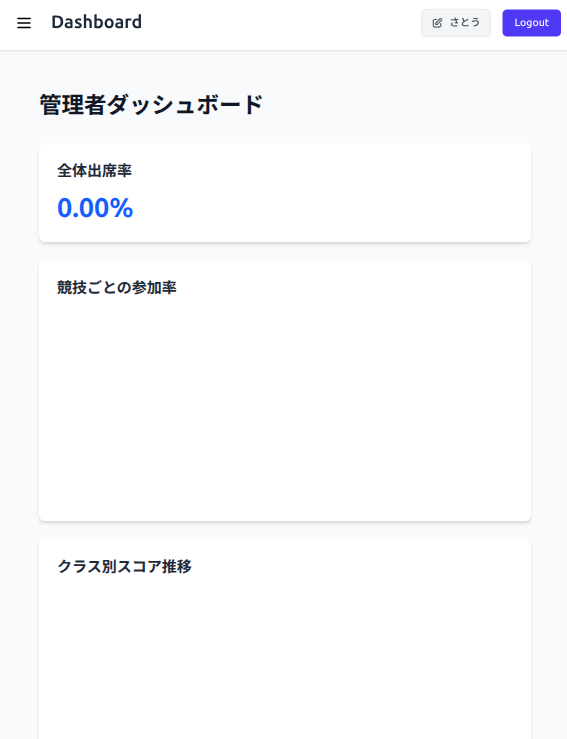
\includegraphics[width=0.8\textwidth]{./images/admin-dashboard.png}
  \caption{行事委員用ダッシュボード}
\end{figure}

\subsection{表示される統計情報}

以下の集計データを一覧で確認できる。

\begin{itemize}
  \item \textbf{出席率} ── クラスごとの出席状況の集計
  \item \textbf{競技別参加率} ── 各スポーツへの参加割合
  \item \textbf{クラス別スコア推移} ── 得点の推移グラフ
  \item \textbf{イベント進捗状況} ── 現在進行中の試合・残り試合数など
\end{itemize}

ダッシュボードは、試合進行中の全体状況を確認するために使用する。
値が想定と異なる場合は、出席管理、チーム編成、試合結果入力のいずれかが未登録または誤登録の可能性がある。
更新直後に表示が変わらない場合は、画面を再読み込みして最新状態を確認する。

\newpage

% =====================================================================
\section{クラス・チーム管理}
% =====================================================================

\textbf{ページ}: \code{/dashboard/admin/class-management}

各クラスのチーム編成を管理する機能である。

\begin{figure}[H]
  \centering
  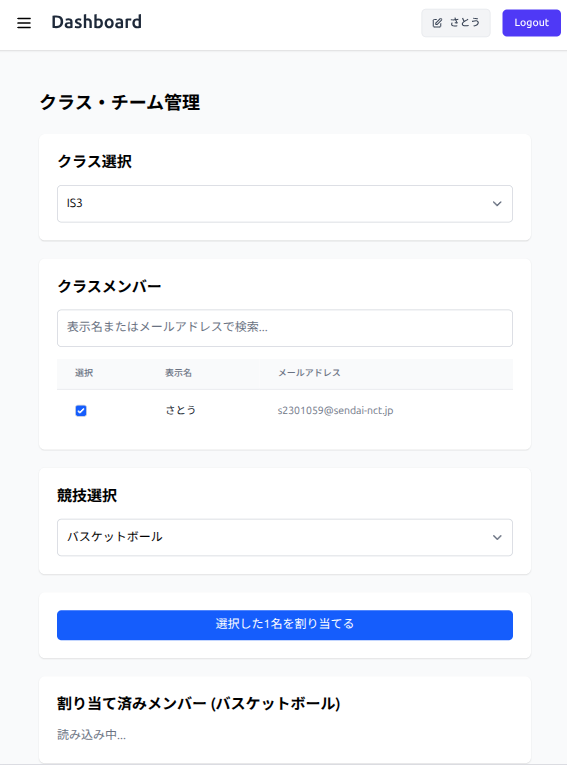
\includegraphics[width=0.8\textwidth]{./images/admin-classmember-manage.png}
  \caption{クラス・チーム管理画面}
\end{figure}

\subsection{担当クラスの確認}

自分が担当するクラスの情報を確認する。
クラス所属ロール（\code{クラス名\_rep}）が割り当てられたクラスが対象となる。
担当クラスが表示されない場合は、rootまたはadminにロール付与状況を確認する。

\subsection{チームメンバーの割り当て}

競技ごとに参加するチームメンバーを登録する。
クラスの学生一覧からメンバーを選択し、チームに割り当てる。
競技ごとの最低定員・最高定員を確認し、必要人数を満たすように登録する。
同じ学生が複数競技に参加する場合は、当日の時間割と重複していないか確認する。

\subsection{チームメンバーの削除}

割り当て済みのメンバーをチームから外すことができる。
大会開始後の削除は、試合進行やMyID参加本登録に影響する可能性があるため、担当者間で確認してから行う。

\subsection{参加本登録済みメンバーの確認}

MyIDバーコード読み取りによって参加本登録されたメンバーの一覧を競技ごとに確認できる。

\newpage

% =====================================================================
\section{ロール管理}\label{sec:role}
% =====================================================================

\textbf{ページ}: \code{/dashboard/admin/role-management}

審判ロールなど、イベント運営上動的に設定する必要がある任意のロールを管理する機能である。

\begin{figure}[H]
  \centering
  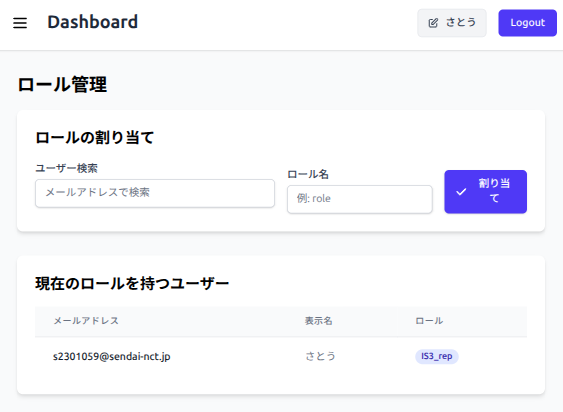
\includegraphics[width=0.8\textwidth]{./images/admin-role-manage.png}
  \caption{ロール管理画面}
\end{figure}

\subsection{ロールの付与}

対象ユーザーを検索し、任意のロールを付与する。
この画面では \code{root} / \code{admin} / \code{student} の基本権限は操作できない。
審判、受付、競技担当など、一時的に必要な任意ロールを付与する。
ロール名は運用上の意味が分かる名前にし、同じ用途で複数の表記を作らないようにする。

\subsection{ロールの削除}

付与済みのロールを削除する。
なお、\code{クラス名\_rep} や \code{クラス名\_競技名} のようなクラス管理ロールは
この画面では削除できない。

\newpage

% =====================================================================
\section{MyIDバーコード読み取り・参加本登録}\label{sec:myid}
% =====================================================================

\subsection{MyIDバーコード読み取り}

\textbf{ページ}: \code{/dashboard/admin/barcode-reader}

学生証等のMyIDバーコードを読み取り、競技への参加本登録とラウンドチェックインを行う機能である。
MyIDは \code{H10} に7桁の学籍番号が続く形式（例: \code{H102301059}）として扱われる。
読み取った学籍番号は、\code{s<学籍番号>@sendai-nct.jp} 形式のメールアドレスを持つユーザーと照合される。

\begin{enumerate}
  \item 「競技」を選択する。
  \item 選択した競技の試合一覧から、受付対象の「試合」を選択する。
        例として、バスケットボールの第1試合を選択すると、バスケットボールの第1ラウンドとしてチェックインされる。
  \item 「読み取り開始」を押し、カメラで学生のMyIDバーコードを読み取る。
  \item カメラが使えない場合は、「手入力」にMyID値を入力して「チェックインする」を押す。
  \item 読み取りに成功すると、参加本登録とラウンドチェックインが完了する。
\end{enumerate}

選択した試合が対象イベント・対象競技に存在しない場合は登録できない。
また、対象学生がその競技に事前エントリーされていない場合も登録できない。
ラウンド番号は手入力せず、選択した試合のトーナメント情報から自動的に決定される。
そのため、事前に対象イベントのトーナメントを生成しておく必要がある。

\begin{center}
\begin{tabular}{p{4.2cm}p{8.8cm}}
\toprule
\textbf{読み取りできない場合} & \textbf{確認すること} \\
\midrule
カメラが起動しない & ブラウザのカメラ権限、端末のカメラ使用可否、HTTPSでアクセスしているかを確認する。 \\
\midrule
該当ユーザーが見つからない & MyIDの学籍番号と、登録メールアドレス \code{s<学籍番号>@sendai-nct.jp} が一致しているか確認する。 \\
\midrule
登録できない & 対象競技への事前エントリー、選択した試合、トーナメント生成状況を確認する。 \\
\bottomrule
\end{tabular}
\end{center}

\subsection{参加本登録済み一覧}

\textbf{ページ}: \code{/dashboard/admin/confirmed-participants}

MyIDバーコード読み取りによって参加本登録された学生の一覧を表示する。
クラスおよび競技ごとにフィルタリングして確認できる。
受付終了後にこの一覧を確認し、参加予定者と読み取り済み人数に差がないか確認する。

\newpage

% =====================================================================
\section{出席管理}\label{sec:attendance}
% =====================================================================

\textbf{ページ}: \code{/dashboard/admin/attendance-management}

各クラスの出席者数を登録・管理する機能である。

\begin{figure}[H]
  \centering
  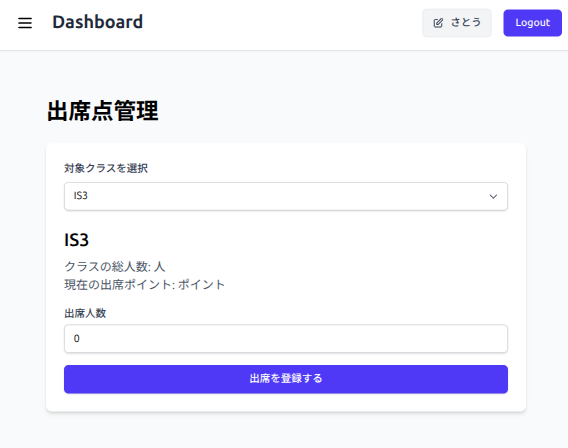
\includegraphics[width=0.8\textwidth]{./images/admin-attend-manage.png}
  \caption{出席管理画面}
\end{figure}

\subsection{出席者数の登録}

クラスを選択し、出席者数を入力して登録する。
登録された数値は統計ダッシュボードや参加率の計算に使用される。
出席者数はクラス全体の人数を超えないように入力する。
点呼後に欠席・早退が判明した場合は、同じ画面から最新の人数に更新する。

\subsection{クラス別出席状況の確認}

クラスごとの出席詳細を参照できる。

\newpage

% =====================================================================
\section{競技詳細登録}
% =====================================================================

\textbf{ページ}: \code{/dashboard/admin/sport-details-registration}

大会に割り当てられた各競技の詳細情報を登録・更新する機能である。

\begin{figure}[H]
  \centering
  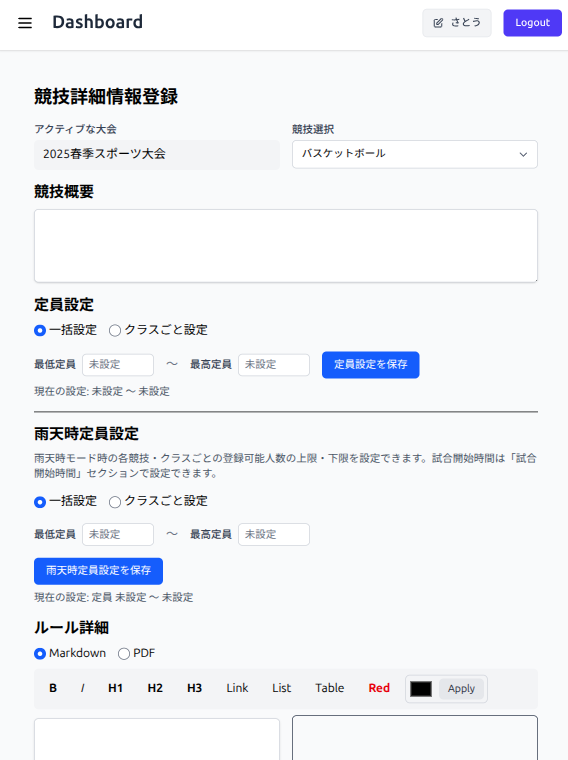
\includegraphics[width=0.8\textwidth]{./images/admin-sports-detail.png}
  \caption{競技詳細登録画面}
\end{figure}

\subsection{競技概要・ルールの登録}

競技の説明やルールをMarkdown形式で記述・更新する。
PDFファイルによる競技要項のアップロードも可能である。
学生の競技情報画面にも表示されるため、集合場所、持ち物、禁止事項など当日必要な情報を含める。

\subsection{定員の設定}

競技全体の最低定員・最高定員を設定する。
クラスごとの定員を個別に設定することもできる。
MyID読み取りによる参加本登録の確認にも利用されるため、実際の競技ルールに合わせて設定する。

\subsection{試合開始時間の設定}

通常時および雨天時の試合開始時間を設定する。
雨天時の開始時間は、rootが雨天時モードをONにした場合に参照される。
通常時と雨天時で場所や時間が変わる競技は、事前に両方の設定を確認しておく。

\begin{figure}[H]
  \centering
  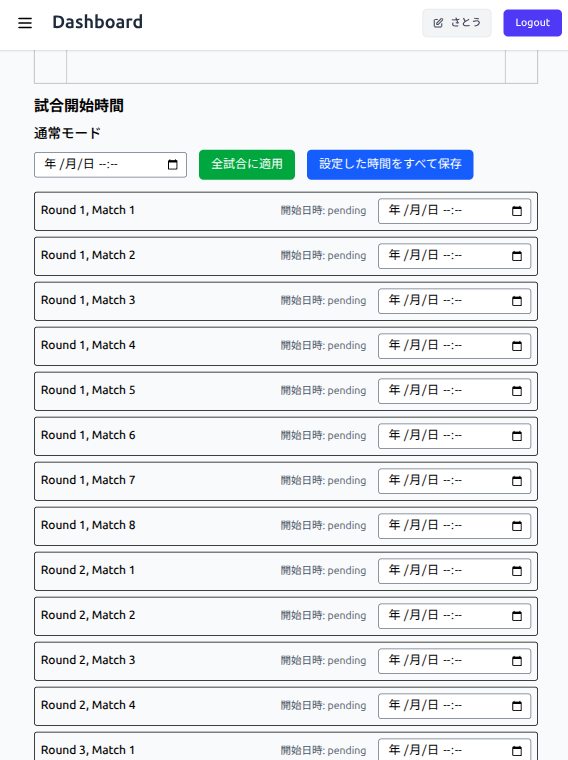
\includegraphics[width=0.8\textwidth]{./images/admin-sports-detail-start-time.png}
  \caption{試合開始時間の設定}
\end{figure}

\newpage

% =====================================================================
\section{試合結果入力}\label{sec:match}
% =====================================================================

\textbf{ページ}: \code{/dashboard/admin/insert-matche-result}

トーナメントの各試合について、進行状況と結果を入力する機能である。

\begin{figure}[H]
  \centering
  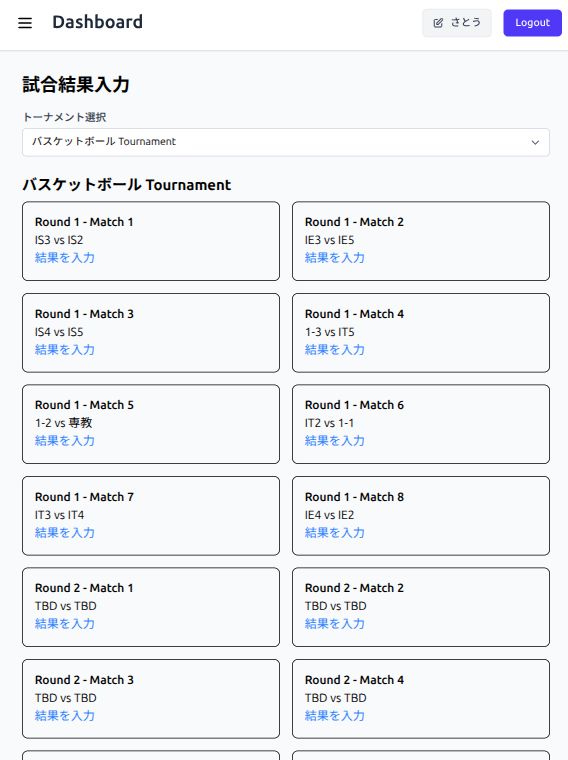
\includegraphics[width=0.8\textwidth]{./images/admin-set-match-score-screen.png}
  \caption{試合結果入力画面}
\end{figure}

\subsection{試合ステータスの更新}

試合ごとに以下のステータスを設定する。

\begin{center}
\begin{tabular}{lp{9cm}}
\toprule
\textbf{ステータス} & \textbf{説明} \\
\midrule
予定 & 試合がまだ始まっていない状態。 \\
進行中 & 試合が現在行われている状態。 \\
終了 & 試合が完了し結果が確定した状態。 \\
\bottomrule
\end{tabular}
\end{center}

試合開始時に「進行中」、結果確定後に「終了」へ変更する。
ステータスは学生のトーナメント・タイムテーブルにも影響するため、入力遅れがないようにする。

\subsection{試合開始時間の更新}

試合の開始時間を変更する場合に更新する。

\subsection{試合結果の入力}

試合終了後、各チームのスコアや勝敗を入力する。
入力された結果はトーナメントブラケットに即時反映される。
入力前に、対戦カードが実際の試合と一致していることを確認する。
スコア入力後は、勝者が次ラウンドへ正しく進んでいるかトーナメント表示で確認する。

\begin{figure}[H]
  \centering
  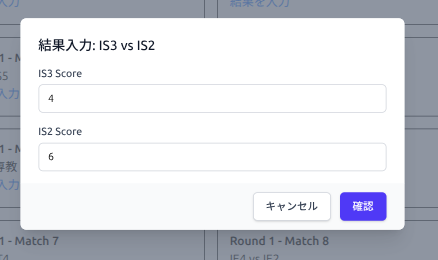
\includegraphics[width=0.8\textwidth]{./images/admin-set-match-score.png}
  \caption{試合結果入力}
\end{figure}

同点の場合でも、勝者を設定することができる。
同点で勝者を決める場合は、競技ルール上の判定方法を確認し、審判の判断に従って入力する。

\begin{figure}[H]
  \centering
  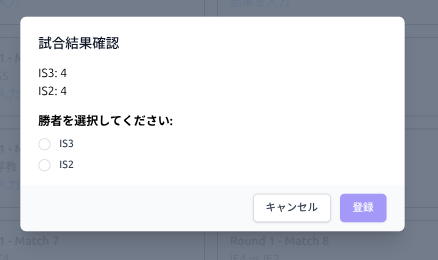
\includegraphics[width=0.8\textwidth]{./images/admin-set-match-score-same-score.png}
  \caption{同点時の点数入力}
\end{figure}

\newpage

% =====================================================================
\section{昼競技（Noon Game）結果入力}\label{sec:noon}
% =====================================================================

\textbf{ページ}: \code{/dashboard/admin/noon-game-results}

昼休みに行われる特別競技（昼競技）の結果を入力する機能である。

\begin{figure}[H]
  \centering
  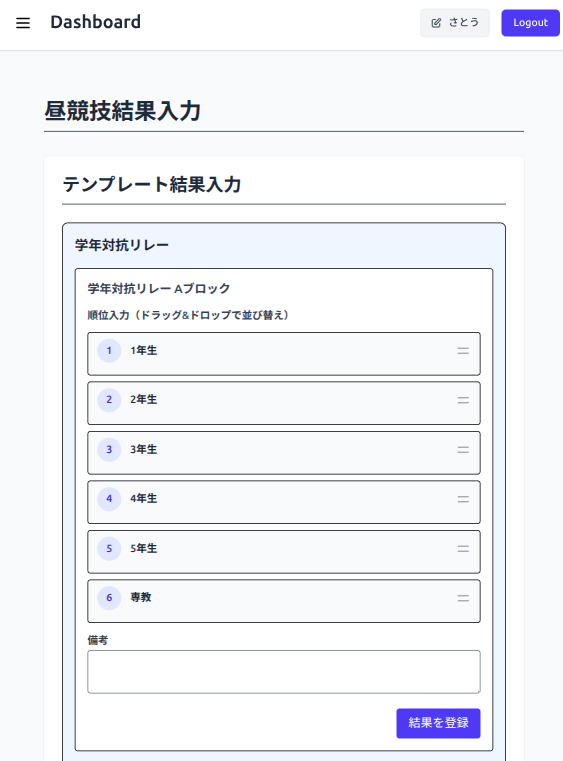
\includegraphics[width=0.8\textwidth]{./images/admin-noon-game-set-score.png}
  \caption{昼競技結果入力}
\end{figure}

\subsection{通常マッチの結果入力}

昼競技の通常試合について、試合結果を入力する。
勝敗または得点を登録すると、クラス別ポイントに反映される。
誤入力に気付いた場合は、同じ試合の結果を修正し、ポイント集計が更新されたことを確認する。

\subsection{テンプレートランの結果入力}

rootが生成した競技テンプレートに対して、以下の各種結果を入力する。

\begin{itemize}
  \item \textbf{年リレー} ── ブロックごとの結果と総合ボーナス
  \item \textbf{コースリレー} ── コース別の結果
  \item \textbf{綱引き} ── 各試合の勝敗
\end{itemize}

テンプレートランはrootが事前に生成した対戦カードに対して結果を入力する。
ドラッグ操作で順位を並べる形式の入力がある場合は、保存前に順位順が正しいか確認する。

\newpage

% =====================================================================
\section{MIC投票}\label{sec:mic}
% =====================================================================

\textbf{ページ}: \code{/dashboard/admin/vorting-mic}

MIC（Most Impressive Class：最も印象を残したクラス）の投票を行う機能である。

\begin{figure}[H]
  \centering
  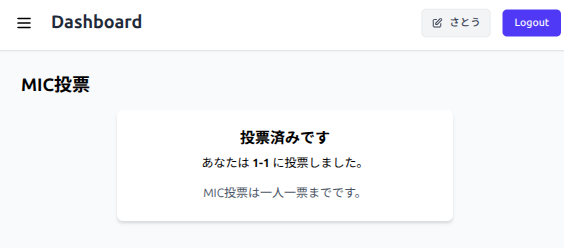
\includegraphics[width=0.8\textwidth]{./images/admin-mic.png}
  \caption{MIC投票}
\end{figure}

\subsection{投票対象クラスの確認}

投票対象となる候補クラスの一覧を確認する。

\subsection{投票の実施}

候補クラスの中から1つを選択して投票する。
投票は1アカウントにつき1票のみ有効である。
投票後の変更可否は画面の状態に従う。
大会運営として不適切な投票を避けるため、判断基準を事前に共有しておく。

\subsection{投票結果の確認}

自分が投票した内容および全体の投票状況を確認できる。
なお、最終的なMIC決定はrootが確認・公表する。

\newpage

% =====================================================================
\section{機能一覧まとめ}
% =====================================================================

以下にadmin権限で実行可能な操作を一覧にまとめる。

\begin{longtable}{p{4.5cm}p{9cm}}
\toprule
\textbf{機能} & \textbf{概要} \\
\midrule
\endhead
管理者ダッシュボード閲覧 & 出席率・参加率・スコア推移・イベント進捗をリアルタイムで確認 \\
\midrule
チームメンバー割り当て & 競技ごとに参加メンバーをクラスから選択して登録・削除 \\
\midrule
ロール付与・削除 & 審判ロールなど任意のロールを学生に付与または削除 \\
\midrule
MyIDバーコード読み取り & 学生のMyIDバーコードを読み取り、参加本登録とラウンドチェックインを実施 \\
\midrule
参加本登録済み一覧の確認 & MyID読み取り済み学生の一覧をクラス・競技別に確認 \\
\midrule
出席者数の登録 & クラスごとの出席者数を入力して登録 \\
\midrule
競技詳細の登録・更新 & 競技のルール・定員・開始時間を設定 \\
\midrule
試合ステータスの更新 & 各試合の進行状況（予定・進行中・終了）を変更 \\
\midrule
試合結果の入力 & トーナメント試合のスコアおよび勝敗を入力 \\
\midrule
昼競技結果の入力 & 昼競技（年リレー・コースリレー・綱引き等）の結果を登録 \\
\midrule
MIC投票 & Most Impressive Classの候補クラスに投票 \\
\bottomrule
\end{longtable}

\end{document}
